\documentclass{article}
\usepackage[utf8]{inputenc}
\usepackage{amsmath}
\usepackage{tikz}

\begin{document}
	
	Temos o problema de contorno definido por, para $ (x, y) \in (0, 1)^2 $ , \\
	\begin{gather}
		-\nabla(\kappa\nabla T) = 0 \texttt{;} \\
		T(x, 0) = T(x, 1) = a \texttt{;} \\
		T(0, y) = b \texttt{;} \, -\kappa \frac{\partial T}{\partial x}(1, y) = h(T - T_{\text{out}})\texttt{.}
	\end{gather}

	
	Consider the boundary conditions:
	\begin{align*}
		T(x, 1) &= a \\
		T(0, y) &= b \\
		-\kappa \frac{\partial T}{\partial x}(1, y) &= h(T - T_{\text{out}})
	\end{align*}
	
	\begin{tikzpicture}
		\draw[step=1cm,gray,very thin] (0,0) grid (3,4);
		\draw[thick] (0,0) -- (0,4) -- (3,4) -- (3,0) -- cycle;
		
		\node at (-0.5, 1.5) {$b$};
		\node at (1.5, 4.5) {$a$};
		\node at (1.5, -0.5) {$a$};
		\node at (4.8, 2.5) {$-\kappa \frac{\partial T}{\partial x} = h(T - T_{\text{out}})$};
	\end{tikzpicture}

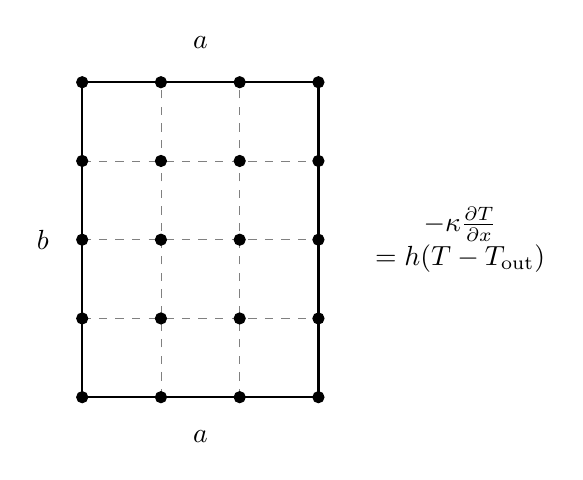
\begin{tikzpicture}
	% Draw a 3x4 grid with dashed lines
	\draw[step=1cm,gray,very thin, dashed] (0,0) grid (3,4);
	
	% Draw the boundary of the grid
	\draw[thick] (0,0) -- (0,4) -- (3,4) -- (3,0) -- cycle;
	
	% Place dots at each intersection of the grid
	\foreach \x in {0,1,2,3}
	\foreach \y in {0,1,2,3,4}
	\filldraw[black] (\x,\y) circle (2pt);
	
	% Add labels next to the grid
	\node at (-0.5, 2) {$b$};
	\node at (1.5, 4.5) {$a$};
	\node at (1.5, -0.5) {$a$};
	\node[align=center] at (4.8, 2) {$-\kappa \frac{\partial T}{\partial x}$ \\ $= h(T - T_{\text{out}})$};
\end{tikzpicture}
	
\end{document}
